\chapter{Background study 802.11}

\section{802.11 header} %changed to header

%\begin{table}[h]
	%	\centering
		%\noindent
		%\small
	%	\begin{tabulary}{1\textwidth}{|C|C|C|C|C|C|C|C|C|C|C|C|}
	%	
	%		\hline
	%			\mc{} & Frame Control & Duration / ID & Address 1 & Address 2 & Address 3 & Sequence Control & Address 4 & QoS Control & HT Control & Frame Body & FCS \\ \hline
	%			\mc{Bytes} & \mc{2} & \mc{2} & \mc{6} & \mc{6} & \mc{6} & \mc{2} & \mc{6} & \mc{2} & \mc{4} & \mc{0-7951} & \mc{4} \\
	%	\end{tabulary}
%		\caption{802.11 MAC frame format}
%\end{table}

\begin{figure}[H]
    \centering
    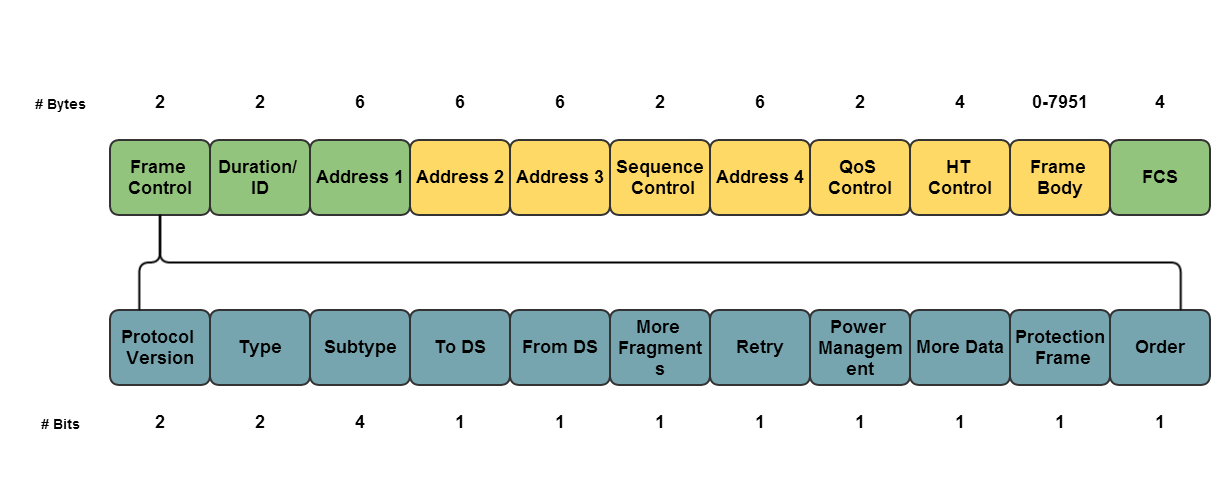
\includegraphics[width=1\textwidth]{figures/80211macframe}
    \caption{802.11 MAC frame} 
    \label{fig:80211macframe_bg}
\end{figure}


\subsection{Frame Control}

In this section a closer look will be taken at the Frame Control. This part is a requirement in every 802.11 MAC frame and will be carefully analyzed. 

\subsubsection{Protocol Version}

This first field consists of 2 bits and is currently always 00. The field is fully reserved for future revisions of the 802.11 header. This field will always stay 00 in the current version of the SHIM DIF.

\subsubsection{Type \& Subtype}

Two fields that consist of 2 and 4 bits. The combination of these two fields determines the function of the current frame. Currently 3 different types are used as type field, these are: 
\begin{itemize}
	\item Management
	\item Control
	\item Data
\end{itemize}

Since these fields are used to set up communication between two devices these fields won't be touched on in the SHIM DIF. Further information on these fields can be found in the IEEE Std. 2012~\citep{ieee80211std}

\subsubsection{To DS \& From DS}

The next two fields are fairly self-explanatory. They decide whether a packet is traveling from or towards a Distribution System (DS). When both of these fields are set to 0 it implies that a frame is traveling straight from one STA to another STA without going to a DS first. Both fields on value 1 means that we are using this in mesh mode and the 4 addresses will be used. Since this SHIM DIF should only providing base function for 802.11 this will not be handled further.

\subsubsection{More Fragments}

This one bit field is set to 1 when either data or management frames have more fragments. In all other cases it should be 0.

\subsubsection{Retry}

A one bit field limited to data or management frames. It is set to 1 when this frame is a retransmission, in all other cases it is set to 0.

\subsubsection{Power Management}

This one bit field's value is heavily reliant on the entire frame. For this limited use SHIM DIF the use of this frame should be copied from the 802.11 standard~\citep{ieee80211std}.

\subsubsection{More Data}

Another one bit field with a specific purpose that will be copied from the standard. This field provides information about following frames that are buffered at the AP for this specific STA.

\subsubsection{Protection Frame}

The second to last field in the Frame Control field is like many other fields a 1 bit field. This bit contains information about the Frame Body. When this Frame Body contains information that has been encrypted this field is set to 1. This is however only the case in specific cases and should be carefully analyzed from the standard. An example here is that this field can never be set to 1 when the Frame Body does not contain any data at all.

\subsubsection{Order}

The final bit in the Frame Control field provides two purposes. It can be set to one in either non-QoS frame or in QoS frames. In both the 1 value provides a different use for the system. Since this also has no further use for the SHIM DIF it will not be handled in detail.

\subsection{Duration / ID}

After the Frame Control field we have the second required field to make a valid 802.11 frame. This is the Duration or ID frame. The frame is 2 bytes (16 bits) large and can be used in various ways. This field is dependent on the type and subtype field earlier mentioned in the Frame Control field. It provides information for the total duration of the frame or provides an ID that can be used to identify and order the frame in it's rightful order. 

\subsection{Address 1, 2, 3 \& 4}

These 4 address fields all use the same type of address fields used in other Ethernet MAC frames. They consist of 6 bytes (48 bits) each and only address 1 most be filled in to complete a valid frame. The addresses can be used for following purposes:

\begin{description}
	\item[BSSID] Basis Service Set Identifier 
	\item[SA] Source Address
	\item[DA] Destination Address
	\item[TA] Transmitting STA Address
	\item[RA] Receiving STA Address
\end{description}

These fields are to be used as the points of attachment MAC addresses of the underlying interfaces. The shim DIF is bound to these interfaces through this address. 

\subsection{Sequence Control}

A 2 byte field that is split up in 2 subfields. Note that this field is not present in control frames, only in data and management ones. The first subfield is the fragment number and is 4 bits long. This subfield tells the fragment number of the frame, starting at 0 for the very first piece and incrementing by 1 step for every consequent fragment. The second subfield is 12 bits long and is the sequence number subfield. This number is the order of the frames and provides information towards the system about the order of frames.

\subsection{QoS Control}


This field provides information about QoS (Quality of Service) settings the frame currently provides. The 16 bit value is dependent on the type, subtype and the transmitting STA of the frame. QoS Control field is needed when the QoS bit in the subtype of a frame is set to 1. The field often contains information about Traffic Identifiers (TID), ACK policy, EOSP, \ldots. A closer look in at these different fields can be taken in the 802.11 standard document~\citep{ieee80211std} (p389). 

\subsection{HT Control}

The final field before the actual frame body is a 4 byte field. The field contains information about the High Throughput of the frame. It is present in Control Wrapper frames and QoS data frames. Since this has little use in RINA it will left as it is and copied exactly from the current standard~\citep{ieee80211std}.

\subsection{Frame Body}

This field is between 0 and 7951 bytes long and contains the actual body of the frame. This will contain further DIFs and ultimately the actual data is should be transferred. Notice that for some frames this can actually be 0, this implies it can be an optional field.

\subsection{FCS}

Final field of the 802.11 frame is a 4byte long Frame Control Sequence. It contains a 32 bit CRC calculated over the entire MAC frame, including the body. The use of this field is to detect errors in the entire frame. It should be copied exactly for the SHIM DIF usage.
